
\documentclass{article}

\usepackage{amsmath}
\usepackage{comment}
\usepackage{amscd}
\usepackage[tableposition=top]{caption}
\usepackage{ifthen}
\usepackage[utf8]{inputenc}

\usepackage{Sweave}
\begin{document}

\title{A DualBrothers Demo}
\maketitle

This is a demo for using the java program, DualBrothers, in R.  To
get started, install the dualbrothers R package from the directory that contains the dualbrothers\_0.0-1.tar.gz file. The rJava package will need to be installed.
\begin{verbatim}
R CMD INSTALL dualbrothers
\end{verbatim}

Start R and load the dualbrothers library.

\begin{Schunk}
\begin{Sinput}
> library(dualbrothers)
\end{Sinput}
\end{Schunk}

Copy the KAL153.phy file from the rbrothers package to your current working directory.
\begin{Schunk}
\begin{Sinput}
> my.align = read.dna(file=system.file("extdata/KAL153/KAL153.phy",package="rbrothers"))
> write.dna(my.align,"KAL153.phy")
\end{Sinput}
\end{Schunk}

Now you can run dualbrothers with a single command.
\begin{Schunk}
\begin{Sinput}
> db<-dualbrothers(123,"KAL153",format="interleaved")
\end{Sinput}
\end{Schunk}

Plots can be created with the following commands.
\begin{Schunk}
\begin{Sinput}
> plot(db,TRUE)
> plottree.db(db,12,TRUE)
\end{Sinput}
\end{Schunk}

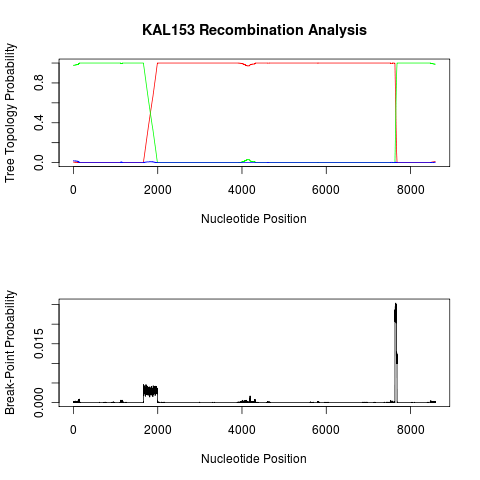
\includegraphics[width=70mm]{KAL153plot1.png}
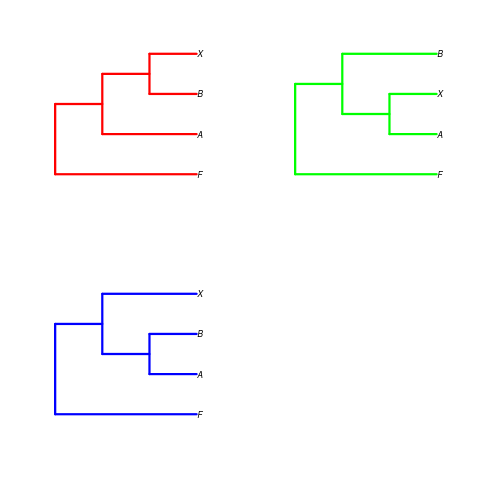
\includegraphics[width=70mm]{KAL153plot2.png}


\end{document}

